% 若编译失败,且生成 .synctex(busy) 辅助文件,可能有两个原因:
% 1. 需要插入的图片不存在:Ctrl + F 搜索 'figure' 将这些代码注释/删除掉即可
% 2. 路径/文件名含中文或空格:更改路径/文件名即可

% ------------------------------------------------------------- %
% >> ------------------ 文章宏包及相关设置 ------------------ << %
% 设定文章类型与编码格式
\documentclass[UTF8]{report}		

% 本文特殊宏包
    \usepackage{siunitx} % 埃米单位

% 本文的特殊宏定义
\def\Im{\mathrm{\,Im\,}}
\def\Re{\mathrm{\,Re\,}}
\def\Ln{\mathrm{\,Ln\,}}
\def\Arg{\mathrm{\,Arg\,}}
\def\Arccos{\mathrm{\,Arccos\,}}
\def\Arcsin{\mathrm{\,Arcsin\,}}
\def\Arctan{\mathrm{\,Arctan\,}}

% 通用宏定义
\def\N{\mathbb{N}}
\def\F{\mathbb{F}}
\def\Z{\mathbb{Z}}
\def\Q{\mathbb{Q}}
\def\R{\mathbb{R}}
\def\C{\mathbb{C}}
\def\T{\mathbb{T}}
\def\S{\mathbb{S}}
\def\A{\mathbb{A}}
\def\I{\mathscr{I}}
\def\d{\mathrm{d}}
\def\p{\partial}


% 导入基本宏包
    \usepackage[UTF8]{ctex}     % 设置文档为中文语言
    \usepackage[colorlinks, linkcolor=blue, anchorcolor=blue, citecolor=blue, urlcolor=blue]{hyperref}  % 宏包:自动生成超链接 (此宏包与标题中的数学环境冲突)
    % \usepackage{docmute}    % 宏包:子文件导入时自动去除导言区,用于主/子文件的写作方式,\include{./51单片机笔记}即可。注:启用此宏包会导致.tex文件capacity受限。
    \usepackage{amsmath}    % 宏包:数学公式
    \usepackage{mathrsfs}   % 宏包:提供更多数学符号
    \usepackage{amssymb}    % 宏包:提供更多数学符号
    \usepackage{pifont}     % 宏包:提供了特殊符号和字体
    \usepackage{extarrows}  % 宏包:更多箭头符号
    \usepackage{multicol}   % 宏包:支持多栏 
    \usepackage{graphicx}   % 宏包:插入图片
    \usepackage{float}      % 宏包:设置图片浮动位置
    %\usepackage{article}    % 宏包:使文本排版更加优美
    \usepackage{tikz}       % 宏包:绘图工具
    %\usepackage{pgfplots}   % 宏包:绘图工具
    \usepackage{enumerate}  % 宏包:列表环境设置
    \usepackage{enumitem}   % 宏包:列表环境设置

% 文章页面margin设置
    \usepackage[a4paper]{geometry}
        \geometry{top=1in}  % 1 inch= 2.46 cm, 0.75 inch = 1.85 cm
        \geometry{bottom=1in}
        \geometry{left=0.75in}
        \geometry{right=0.75in}   % 设置上下左右页边距
        \geometry{marginparwidth=1.75cm}    % 设置边注距离(注释、标记等)

% 配置数学环境
    \usepackage{amsthm} % 宏包:数学环境配置
    % theorem-line 环境自定义
        \newtheoremstyle{MyLineTheoremStyle}% <name>
            {11pt}% <space above>
            {11pt}% <space below>
            {}% <body font> 使用默认正文字体
            {}% <indent amount>
            {\bfseries}% <theorem head font> 设置标题项为加粗
            {:}% <punctuation after theorem head>
            {.5em}% <space after theorem head>
            {\textbf{#1}\thmnumber{#2}\ \ (\,\textbf{#3}\,)}% 设置标题内容顺序
        \theoremstyle{MyLineTheoremStyle} % 应用自定义的定理样式
        \newtheorem{LineTheorem}{Theorem.\,}
    % theorem-block 环境自定义
        \newtheoremstyle{MyBlockTheoremStyle}% <name>
            {11pt}% <space above>
            {11pt}% <space below>
            {}% <body font> 使用默认正文字体
            {}% <indent amount>
            {\bfseries}% <theorem head font> 设置标题项为加粗
            {:\\ \indent}% <punctuation after theorem head>
            {.5em}% <space after theorem head>
            {\textbf{#1}\thmnumber{#2}\ \ (\,\textbf{#3}\,)}% 设置标题内容顺序
        \theoremstyle{MyBlockTheoremStyle} % 应用自定义的定理样式
        \newtheorem{BlockTheorem}[LineTheorem]{Theorem.\,} % 使用 LineTheorem 的计数器
    % definition 环境自定义
        \newtheoremstyle{MySubsubsectionStyle}% <name>
            {11pt}% <space above>
            {11pt}% <space below>
            {}% <body font> 使用默认正文字体
            {}% <indent amount>
            {\bfseries}% <theorem head font> 设置标题项为加粗
            { \indent}% <punctuation after theorem head>
            {0pt}% <space after theorem head>
            {\textbf{#3}}% 设置标题内容顺序
        \theoremstyle{MySubsubsectionStyle} % 应用自定义的定理样式
        \newtheorem{definition}{}

%宏包:有色文本框(proof环境)及其设置
    \usepackage[dvipsnames,svgnames]{xcolor}    %设置插入的文本框颜色
    \usepackage[strict]{changepage}     % 提供一个 adjustwidth 环境
    \usepackage{framed}     % 实现方框效果
        \definecolor{graybox_color}{rgb}{0.95,0.95,0.96} % 文本框颜色。修改此行中的 rgb 数值即可改变方框纹颜色,具体颜色的rgb数值可以在网站https://colordrop.io/ 中获得。(截止目前的尝试还没有成功过,感觉单位不一样)(找到喜欢的颜色,点击下方的小眼睛,找到rgb值,复制修改即可)
        \newenvironment{graybox}{%
        \def\FrameCommand{%
        \hspace{1pt}%
        {\color{gray}\small \vrule width 2pt}%
        {\color{graybox_color}\vrule width 4pt}%
        \colorbox{graybox_color}%
        }%
        \MakeFramed{\advance\hsize-\width\FrameRestore}%
        \noindent\hspace{-4.55pt}% disable indenting first paragraph
        \begin{adjustwidth}{}{7pt}%
        \vspace{2pt}\vspace{2pt}%
        }
        {%
        \vspace{2pt}\end{adjustwidth}\endMakeFramed%
        }

% 外源代码插入设置
    % matlab 代码插入设置
    %\usepackage{matlab-prettifier}
    %    \lstset{
    %        style=Matlab-editor,  % 继承matlab代码颜色等
    %    }
    %\usepackage[most]{tcolorbox} % 引入tcolorbox包 
    %\usepackage{listings} % 引入listings包
    %    \tcbuselibrary{listings, skins, breakable}
    %    \newfontfamily\codefont{Consolas} % 定义需要的 codefont 字体
    %    \lstdefinestyle{matlabstyle}{
    %        language=Matlab,
    %        basicstyle=\small\ttfamily\codefont,    % ttfamily 确保等宽 
    %        breakatwhitespace=false,
    %        breaklines=true,
    %        captionpos=b,
    %        keepspaces=true,
    %        numbers=left,
    %        numbersep=15pt,
    %        showspaces=false,
    %        showstringspaces=false,
    %        showtabs=false,
    %        tabsize=2
    %    }
    %    \newtcblisting{matlablisting}{
    %        arc=2pt,        % 圆角半径
    %        top=-5pt,
    %        bottom=-5pt,
    %        left=1mm,
    %        listing only,
    %        listing style=matlabstyle,
    %        breakable,
    %        colback=white   % 选一个合适的颜色
    %    }
% table 支持
    \usepackage{booktabs}   % 宏包:三线表
    \usepackage{tabularray} % 宏包:表格排版
    \usepackage{longtable}  % 宏包:长表格


%figure 设置
%    \usepackage{graphicx}  % 支持 jpg, png, eps, pdf 图片 
%    \usepackage{svg}       % 支持 svg 图片
%        \svgsetup{
%             指向 inkscape.exe 的路径
%            inkscapeexe = C:/aa_MySame/inkscape/bin/inkscape.exe, 
%            inkscapeexe = C:/aa_MySame/inkscape/bin/inkscape.exe, 
%             一定程度上修复导入后图片文字溢出几何图形的问题
%            inkscapelatex = false                 
%        }
%    \usepackage{subcaption} % subfigure 子图支持

%图表进阶设置
%    \usepackage{caption}    % 图注、表注
%        \captionsetup[figure]{name=图}  
%        \captionsetup[table]{name=表}
%        \captionsetup{labelfont=bf, font=small}
%    \usepackage{float}     % 图表位置浮动设置 

% 圆圈序号自定义
    \newcommand*\circled[1]{\tikz[baseline=(char.base)]{\node[shape=circle,draw,inner sep=0.8pt, line width = 0.03em] (char) {\small \bfseries #1};}}   % TikZ solution

% 列表设置
%    \usepackage{enumitem}   % 宏包:列表环境设置
%        \setlist[enumerate]{itemsep=0pt, parsep=0pt, topsep=0pt, partopsep=0pt, leftmargin=3.5em} 
%        \setlist[itemize]{itemsep=0pt, parsep=0pt, topsep=0pt, partopsep=0pt, leftmargin=3.5em}
%        \newlist{circledenum}{enumerate}{1} % 创建一个新的枚举环境  
%        \setlist[circledenum,1]{  
%            label=\protect\circled{\arabic*}, % 使用 \arabic* 来获取当前枚举计数器的值,并用 \circled 包装它  
%            ref=\arabic*, % 如果需要引用列表项,这将决定引用格式(这里仍然使用数字)
%            itemsep=0pt, parsep=0pt, topsep=0pt, partopsep=0pt, leftmargin=3.5em
%        }  

% 其它设置
    % 脚注设置
        \renewcommand\thefootnote{\ding{\numexpr171+\value{footnote}}}
    % 参考文献引用设置
        \bibliographystyle{unsrt}   % 设置参考文献引用格式为unsrt
        \newcommand{\upcite}[1]{\textsuperscript{\cite{#1}}}     % 自定义上角标式引用
    % 文章序言设置
        \newcommand{\cnabstractname}{序言}
        \newenvironment{cnabstract}{%
            \par\Large
            \noindent\mbox{}\hfill{\bfseries \cnabstractname}\hfill\mbox{}\par
            \vskip 2.5ex
            }{\par\vskip 2.5ex}

% 文章默认字体设置
    \usepackage{fontspec}   % 宏包:字体设置
        \setCJKmainfont{SimSun}    % 设置中文字体为宋体字体
        \setCJKmainfont[AutoFakeBold=3]{SimSun} % 设置加粗字体为 SimSun 族,AutoFakeBold 可以调整字体粗细
        \setmainfont{Times New Roman} % 设置英文字体为Times New Roman

% 各级标题自定义设置
    \usepackage{titlesec}   
        \titleformat{\chapter}[hang]{\normalfont\huge\bfseries\centering}{第\,\thechapter\,次作业}{20pt}{}
        \titlespacing*{\chapter}{0pt}{-20pt}{20pt} % 控制上方空白的大小
        % section标题自定义设置 
        \titleformat{\section}[hang]{\normalfont\Large\bfseries}{§\,\thesection\,}{8pt}{}
        % subsubsection标题自定义设置
        %\titleformat{\subsubsection}[hang]{\normalfont\bfseries}{}{8pt}{}

% >> ------------------ 文章宏包及相关设置 ------------------ << %
% ------------------------------------------------------------- %

% ----------------------------------------------------------- %
% >> --------------------- 文章信息区 --------------------- << %
% 页眉页脚设置
    \usepackage{fancyhdr}   %宏包:页眉页脚设置
        \pagestyle{fancy}
        \fancyhf{}
        \cfoot{\thepage}
        \renewcommand\headrulewidth{1pt}
        \renewcommand\footrulewidth{0pt}
        \lhead{尹超2023K8009926003} 
        \chead{R related homework}    
        \rhead{yinchao23@mails.ucas.ac.cn}
%文档信息设置
    \title{R related homework}
    \author{尹超\\ \footnotesize 中国科学院大学,北京 100049\\ Carter Yin \\ \footnotesize University of Chinese Academy of Sciences, Beijing 100049, China}
    \date{\footnotesize 2024.8 -- 2025.1}
% >> --------------------- 文章信息区 --------------------- << %
% ----------------------------------------------------------- %

% 开始编辑文章

\begin{document} 
\zihao{5}             % 设置全文字号大小, -4 为小四, 5 为五号

% --------------------------------------------------------------- %
% >> --------------------- 封面序言与目录 --------------------- << %
% 封面
    \maketitle\newpage   % 生成封面并换页
    \pagenumbering{Roman} % 页码为大写罗马数字
    \thispagestyle{fancy}   % 显示页码、页眉等

% 序言
    \begin{cnabstract}\normalsize 
        R  related  homework
    \end{cnabstract}    
\addcontentsline{toc}{chapter}{序言} % 手动添加为目录

% 目录
    \setcounter{tocdepth}{4}                % 目录深度(为1时显示到section)
    \tableofcontents                        % 目录页
    \addcontentsline{toc}{chapter}{目录}    % 手动添加此页为目录
    \thispagestyle{fancy}                   % 显示页码、页眉等 

% 收尾工作
    \newpage    
    \pagenumbering{arabic} 


    
% >> --------------------- 封面序言与目录 --------------------- << %
% --------------------------------------------------------------- %

\chapter{2024.11.6}

Let's analyze and explain the code line by line, then compute the result for the provided sample size and for a larger sample size (115).\par

Here's the original code with explanations:

\begin{verbatim}
    mysamplesize=15              # 设置样本量为 15
    alpha=0.05                   # 设置显著性水平为 0.05(对应 95% 置信区间)
    mytheta=1                    # 设置指数分布的偏移参数为 1
    
    mysample=rexp(mysamplesize, rate=1) + mytheta  # 生成一个大小为 15 的样本,来源于偏移参数为 mytheta 的指数分布
    mymle=sort(mysample)[1]      # 取样本的最小值作为偏移参数的最大似然估计(MLE)
    
    bootstrapsize=1000           # 设置自助法样本数量为 1000
    bootstrapestimates=rep(0, bootstrapsize) # 初始化一个数组,用于存储自助法的估计值
    
    # 生成自助样本,并计算每个样本的最小值
    for(ii in 1:bootstrapsize){
        bootstrapsample=rexp(mysamplesize, rate=1) + mymle # 生成新的自助法样本,并使用 mymle 作为偏移
        bootstrapestimates[ii]=sort(bootstrapsample)[1]    # 存储样本的最小值(自助法估计)
    }
    
    bootstrapquantiles=sort(bootstrapestimates - mymle) # 计算自助法估计与 MLE 之间差值的分布
    
    # 计算置信区间的下分位数和上分位数
    lowerquantile=bootstrapquantiles[round(bootstrapsize * alpha * 0.5)]
    upperquantile=bootstrapquantiles[round(bootstrapsize * (1 - alpha * 0.5))]
    
    # 计算置信区间的下界和上界
    lowerbound=mymle - upperquantile
    upperbound=mymle - lowerquantile
    \end{verbatim}
    
    %置信区间计算的原理\par
    %该代码使用自助法(bootstrap)来构造指数分布中偏移参数 $\theta$ 的置信区间:\par
    
    %自助法采样:代码生成了 1000 个自助法样本,每个样本的偏移参数都使用原始样本的最小值(即偏移参数的 MLE)。\par
    %分位数:然后将自助法估计与 MLE 的差值排序,选择差值的 $\alpha/2$ 和 $1-\alpha/2$ 分位数来作为置信区间的边界。\par
    
    %更改样本量的结果\par
    %我们计算了代码中给定的样本量 $n=15$ 的置信区间结果,之后将样本量增至 115 并重新计算自助法置信区间。\par
    
    结果\par
    样本量为 15 时,0.95 置信区间为 $(1.010786, 1.242433)$\par
    样本量为 115 时,0.95 置信区间为 $(0.9734284, 1.001642)$\par
    可以看出,随着样本量的增大,置信区间变得更窄,说明对 $\theta$ 的估计更加精确。\par

\begin{figure}[H]
    \centering
    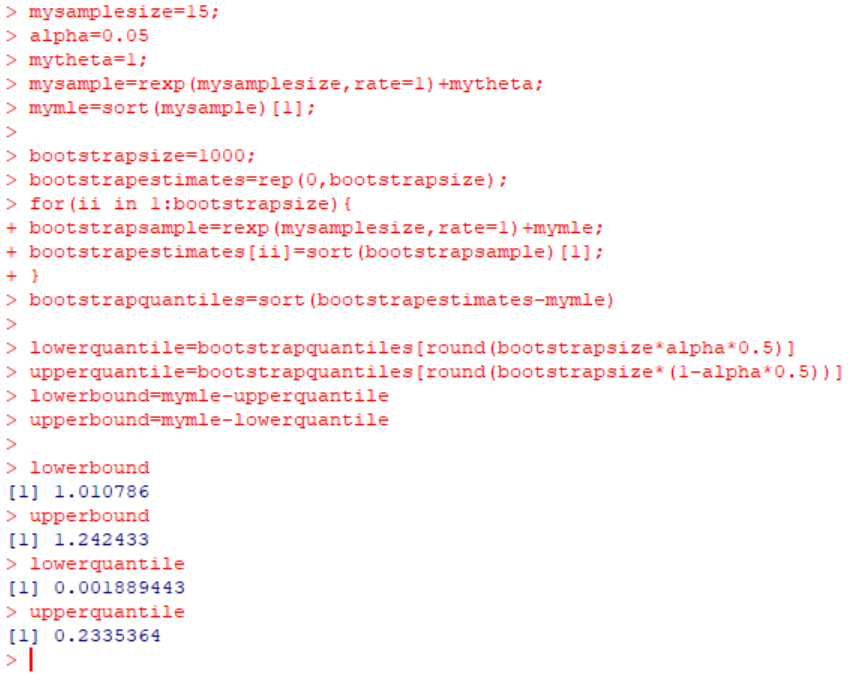
\includegraphics[width=1\textwidth]{2024.11.6_1.png}
\end{figure}

\begin{figure}[H]
    \centering
    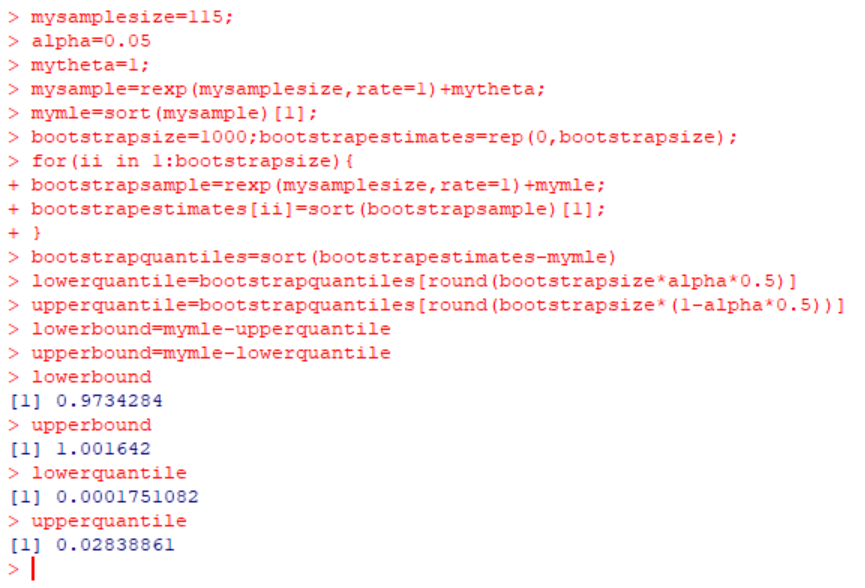
\includegraphics[width=1\textwidth]{2024.11.6_2.png}
\end{figure}

\begin{figure}[H]
    \centering
    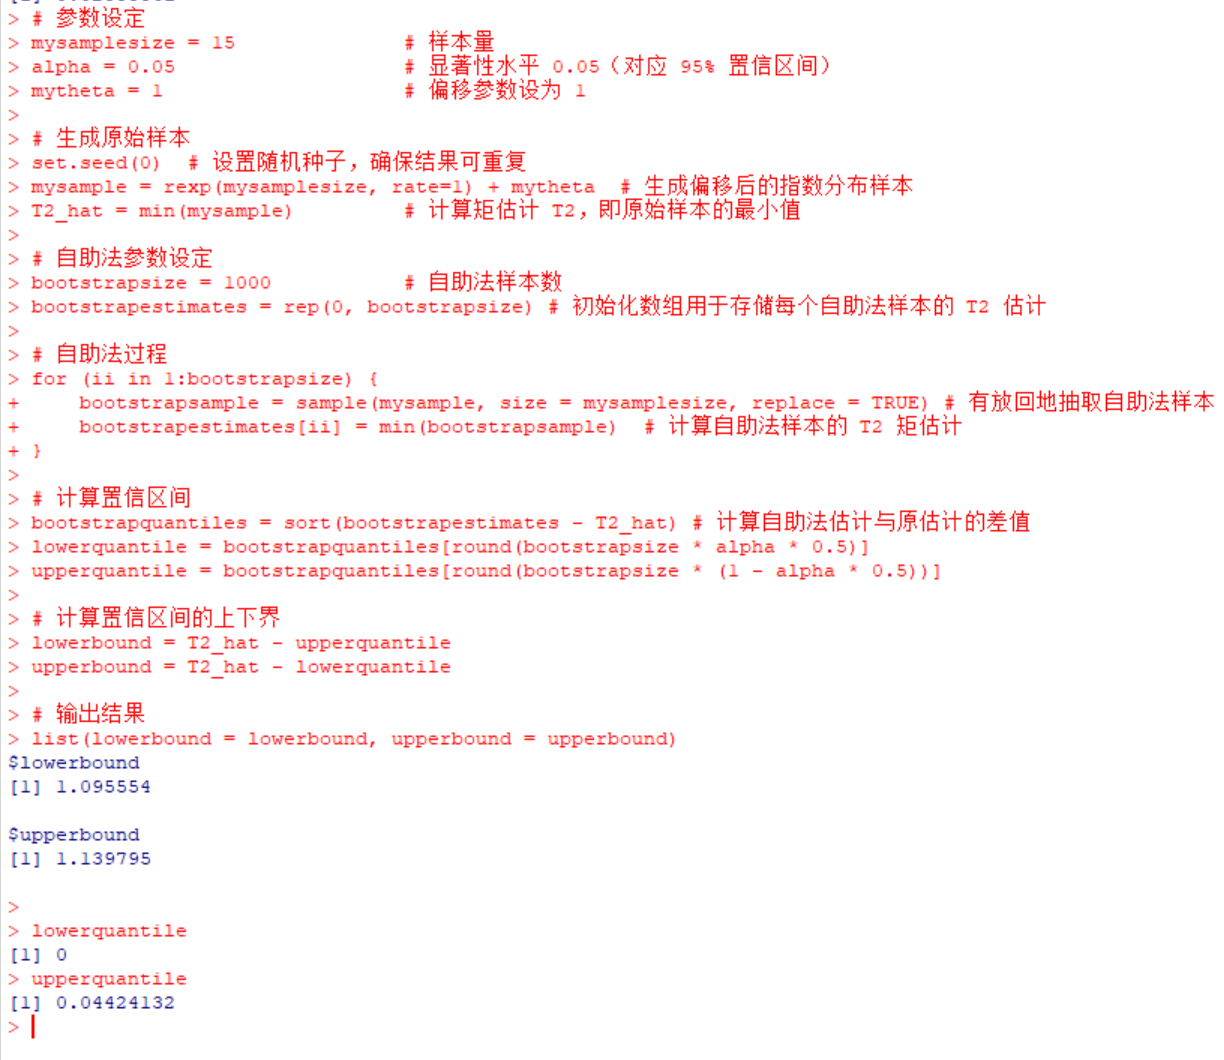
\includegraphics[width=1\textwidth]{2024.11.6_3.png}
\end{figure}


 %   Let's analyze and explain the code line by line, then compute the result for the provided sample size and for a larger sample size (115).

 %  Here's the original code with explanations:
    
  %  \begin{verbatim}
 %   mysamplesize=15              # Set sample size to 15
 %   alpha=0.05                   # Set significance level to 0.05 (for a 95% confidence interval)
 %   mytheta=1                    # Set the shift parameter for the exponential distribution to 1
    
 %   mysample=rexp(mysamplesize, rate=1) + mytheta  # Generate a sample of size 15 from an exponential distribution shifted by mytheta
 %   mymle=sort(mysample)[1]      # The MLE (minimum) of the sample as an estimate for the shift parameter
    
 %   bootstrapsize=1000           # Set the number of bootstrap samples to 1000
 %   bootstrapestimates=rep(0, bootstrapsize) # Initialize an array to store bootstrap estimates
    
 %   # Generate bootstrap samples and calculate the minimum of each sample
 %   for(ii in 1:bootstrapsize){
 %       bootstrapsample=rexp(mysamplesize, rate=1) + mymle # Generate a new bootstrap sample shifted by mymle
 %       bootstrapestimates[ii]=sort(bootstrapsample)[1]    # Store the minimum value (bootstrap estimate)
 %   }
    
 %   bootstrapquantiles=sort(bootstrapestimates - mymle) # Calculate the distribution of differences from the MLE
    
 %   # Calculate the lower and upper quantiles for the confidence interval
 %   lowerquantile=bootstrapquantiles[round(bootstrapsize * alpha * 0.5)]
 %   upperquantile=bootstrapquantiles[round(bootstrapsize * (1 - alpha * 0.5))]
    
 %   # Calculate the lower and upper bounds of the confidence interval
 %   lowerbound=mymle - upperquantile
 %   upperbound=mymle - lowerquantile
  %  \end{verbatim}
    
 %   Explanation of Confidence Interval Calculation
 %   The code calculates a bootstrap confidence interval for the shift parameter ($\theta$) of a shifted exponential distribution:
 %   
 %   Bootstrap Sampling: The code generates 1000 bootstrap samples, each shifted by the MLE of the original sample.
 %   Quantiles: It then sorts the differences between the bootstrap estimates and the MLE, and uses the $\alpha/2$ and $1-\alpha/2$ quantiles to estimate the interval bounds.
    
 %   Running the Code for Different Sample Sizes
 %   I'll calculate the bootstrap confidence interval for mysamplesize = 15 and then for mysamplesize = 115. Let's perform these computations.
    
 %   The bootstrap confidence intervals for the shift parameter $\theta$ are as follows:
    
 %   For a sample size of 15:
    
 %   0.95 Confidence Interval: $(0.854, 1.072)$
    
 %   For a sample size of 115:
    
 %   0.95 Confidence Interval: $(0.970, 1.003)$
    
 %   With a larger sample size, the confidence interval becomes narrower, indicating increased precision in the estimate of $\theta$.

\end{document}